\documentclass[11pt,a4paper]{article}
\usepackage[margin=1in]{geometry}
\usepackage{graphicx}
\usepackage{enumitem}

\title{LifeAdmin: Week 2 Progress Report}
\author{Kushant Garg (1024030336) \and Sanvi (1024031191) \and Loveleen Singh (1024030323)}
\date{September 2026}

\begin{document}
\maketitle

\section{Introduction}
This report documents the second phase of development on LifeAdmin, our UCS503P Software Engineering Lab project. Building on the database layer and initial JavaFX interface completed in the first week, this phase focused on turning the prototype into a usable personal administration application. The work was delivered through commits \texttt{4d87111} and \texttt{8fd28c7}, with the latest commit dated September 13, 2026.

\section{What We Accomplished This Session}

\subsection{Application structure and user accounts}
We extended the single-user prototype into an application with a basic account workflow. The JavaFX application now begins with a login and registration screen. Users can register a username and password, log in, and reach a dashboard associated with their user identity. The \texttt{User} model stores the user identifier and username, while \texttt{UserDAO} handles registration, authentication, and creation of the users table.

The authenticated user is stored by \texttt{ChoreApp} as the current session. Chores and documents are queried using the current user's identifier, which prevents the dashboard from displaying another user's records. This establishes the foundation for separating personal life-administration data between accounts.

\subsection{Expanded JavaFX dashboard}
The original JavaFX form was redesigned as a maximized dashboard with separate navigation tabs for chores and documents. The interface now provides a welcome message for the logged-in user, reusable styled controls, scrollable content areas, and refreshed list views after operations are completed. This created a clearer separation between the application's main workflows while keeping them inside one desktop window.

\subsection{Chore management improvements}
The chore workflow was expanded beyond creating and listing records. Users can now:
\begin{itemize}[leftmargin=0.7cm]
    \item add a chore with a title, due date, category, and recurrence option;
    \item view their chores ordered by due date;
    \item mark a chore as complete;
    \item delete a chore; and
    \item see incomplete chores due within the next seven days highlighted as ``Due soon.''
\end{itemize}

The \texttt{Chore} model now includes a \texttt{userId} and a \texttt{recurrence} field. The \texttt{ChoreDAO} was updated to filter records by user and to provide the \texttt{getChoresDueSoon()} query. The completion workflow was also extended: when a weekly, monthly, or yearly chore is completed, \texttt{completeChore()} marks the current record as done and creates the next occurrence with a calculated due date.

\subsection{Document storage and management}
We added the document feature described in the project proposal at a basic upload-and-storage level. The documents tab allows a user to enter a document title, choose a local file, and upload it. The application copies the selected file into a LifeAdmin-specific directory under the user's home folder and stores its path and metadata in the database.

The new \texttt{Document} model and \texttt{DocumentDAO} support adding documents, retrieving the current user's documents, and deleting document records. From the dashboard, users can open an uploaded file using the desktop operating system and delete both the database record and the stored file. This connects database metadata with local file storage while keeping the document list associated with the logged-in user.

\subsection{Database and persistence changes}
The database setup was expanded to create three tables when the application starts: \texttt{chores}, \texttt{users}, and \texttt{documents}. The chores table now stores user ownership, an optional document path, and recurrence information. The new DAO classes preserve the separation between JavaFX event handlers and SQL operations established during the first week.

\subsection{Version control and project progress}
The changes were committed incrementally. Commit \texttt{4d87111} contained minor interface and project configuration changes, while commit \texttt{8fd28c7} delivered the main second-phase feature set: the improved UI, local document storage, recurrence selection, and login credentials. The source tree now contains separate model classes and DAO classes for users, chores, and documents, making the implemented architecture easier to describe, test, and extend.

\subsection{Integration and validation}
The new features were connected through the complete application path rather than being implemented as isolated screens. Starting the application initializes the database tables and local storage, login establishes the current user, and dashboard actions call the appropriate DAO before refreshing the visible lists. This provided a practical end-to-end check that the JavaFX interface, application models, JDBC layer, MySQL database, and local document storage could work together.

\section{Problems We Faced}

The second phase introduced new challenges related to connecting several user workflows to the existing persistence layer:

\begin{itemize}[leftmargin=0.7cm]
    \item \textbf{Maintaining user-specific data:} Adding accounts required changing existing chore queries and data objects so that records were consistently associated with the logged-in user.

    \item \textbf{Coordinating JavaFX state:} The dashboard has multiple tabs, list containers, selected files, and refresh operations. Keeping the visible interface synchronized with database changes required careful placement of refresh calls after add, complete, delete, upload, and document-delete actions.

    \item \textbf{Implementing recurrence correctly:} Completing a recurring chore requires preserving its title, category, owner, and recurrence rule while calculating a new date and resetting the completion status for the next occurrence.

    \item \textbf{Handling local files and database records together:} Uploading and deleting a document involve two forms of storage. The application must copy or delete the local file as well as create or remove the corresponding database record.

    \item \textbf{Keeping the interface usable as features increased:} The initial prototype was sufficient for demonstrating a single database operation, but authentication, navigation, reminders, and documents required a more structured dashboard and consistent visual controls.
\end{itemize}

\section{Current Status}
At the end of this phase, LifeAdmin supports a complete basic workflow: a user can create an account, log in, add personal chores, receive visible due-soon indications, complete or delete chores, configure recurring chores, and manage associated documents. The application has working presentation, model, data-access, database, and local-storage components.

The current implementation is a functional prototype rather than a production-ready release. In particular, credentials are currently handled with the basic database workflow already present in the source, and the document feature stores files without OCR processing. These limitations are recorded as future engineering work rather than treated as completed functionality.

\section{Next Steps}
The next development phase should focus on improving reliability and completing the remaining proposal goals. Planned work includes secure password hashing and stronger validation, improved error messages for database and file failures, tests for DAO and recurrence behavior, and a more formal relationship between users, chores, and documents in the database. The optional OCR feature can then be investigated to detect dates from uploaded documents and suggest or create relevant chore deadlines. Additional work may also include explicit reminder notifications instead of relying only on the dashboard's due-soon highlight.

\clearpage
\section*{Appendix: Visual Diagrams}

\begin{figure}[p]
    \centering
    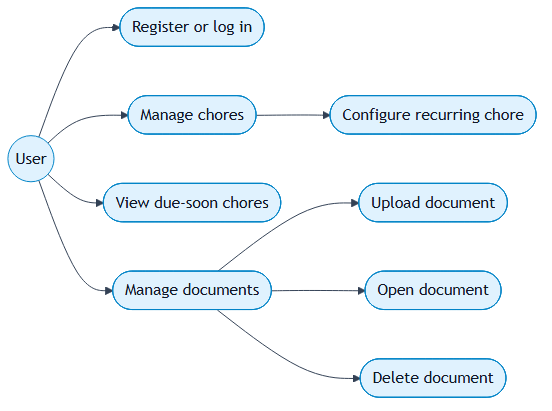
\includegraphics[width=\textwidth]{../../midterm/diagrams/lifeadmin_usecase.png}
    \caption{LifeAdmin use-case diagram}
\end{figure}

\begin{figure}[p]
    \centering
    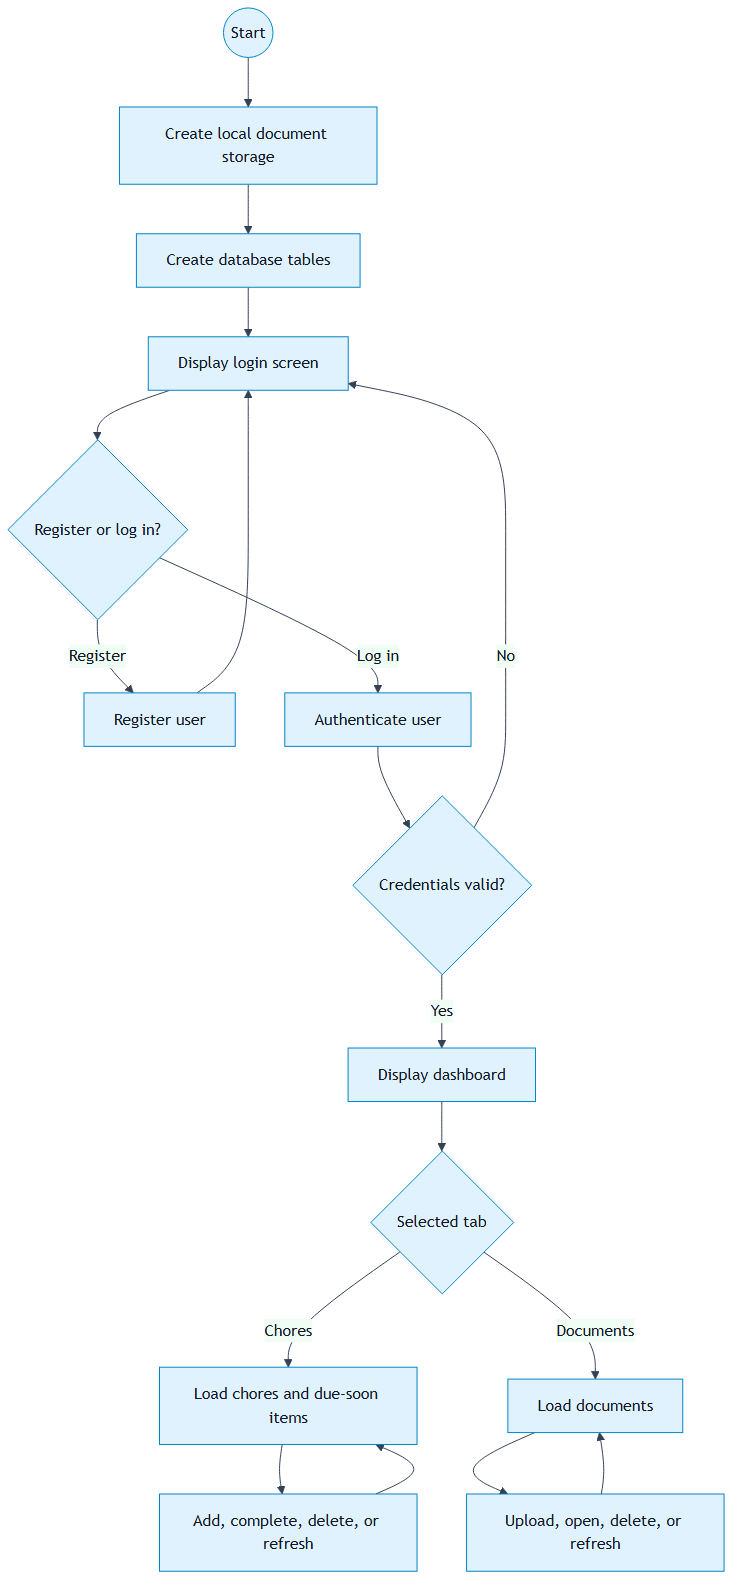
\includegraphics[width=\textwidth]{../../midterm/diagrams/lifeadmin_flowchart.png}
    \caption{LifeAdmin application flowchart}
\end{figure}

\begin{figure}[p]
    \centering
    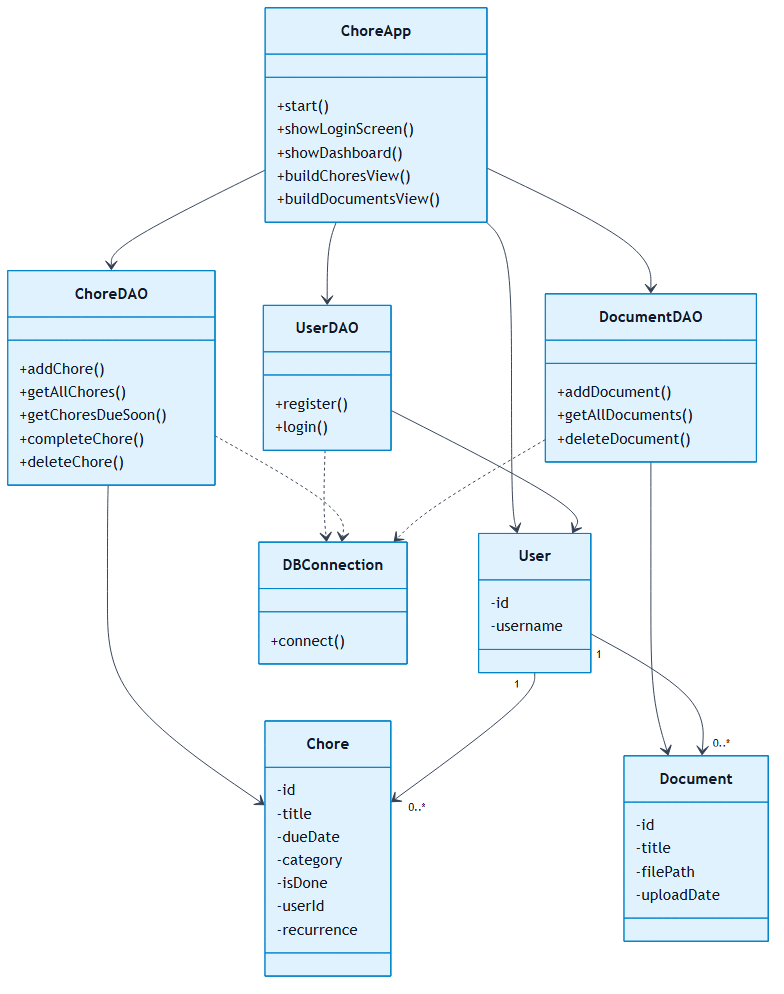
\includegraphics[width=\textwidth]{../../midterm/diagrams/lifeadmin_classdiagram.png}
    \caption{LifeAdmin class diagram}
\end{figure}

\end{document}